\documentclass[11pt,letterpaper]{article}
\usepackage[margin=0.7in]{geometry}
\usepackage[T1]{fontenc}
\usepackage{lmodern,microtype,graphicx,booktabs,amsmath,fancyhdr}
\usepackage[hidelinks]{hyperref}
\usepackage[font=small,labelfont=bf]{caption}
\setlength{\parindent}{0pt}\setlength{\parskip}{7pt}\setlength{\emergencystretch}{4em}
\pagestyle{fancy}\fancyhf{}\fancyhead[L]{Storm-damage ranking sensitivity}
\fancyhead[R]{Independent research manuscript}
\fancyfoot[L]{29 October 2026 --- not peer reviewed}\fancyfoot[R]{\thepage}
\setlength{\headheight}{14pt}
\begin{document}
{\LARGE\bfseries A recorded-damage ranking\\does not identify true storm risk\par}
\vspace{8pt}
{\large Reporting scenarios, tail influence and resampling units in six states\par}
{\small James N. Jean IV \quad Independent, AI-assisted research example \quad 29 October 2026\par}
\section*{Executive summary}
An analyst using storm-damage tables to prioritize further investigation needs to know whether the ordering survives changes in the analysis. This study uses NOAA/NWS reports for five county-designated weather-event types in Illinois, Indiana, Michigan, Minnesota, Ohio and Wisconsin. Scenario thresholds use 2015--2019; the comparison uses the later 2020--2023 period.

The ordering is sensitive to the stated assumptions. Illinois ranges from rank 2 to rank 6 across six fixed blank-value and tail-treatment scenarios. Michigan ranks first in five scenarios but third when the upper blank-value assignment is combined with the tail cap. The uncapped, blank-as-zero comparator gives Michigan a 49.1\% mean annual share of the six-state panel's recorded damage. The combined stress gives it 17.5\%. These scenarios change the accounting estimand; neither is an estimate of true missing loss.

\begin{center}\small
\begin{tabular}{lrrr}\toprule
State & Comparator share & Scenario rank range & Top-two scenarios\\
 & \% & minimum--maximum & out of six\\\midrule
Illinois & 21.4 & 2--6 & 2\\
Indiana & 9.8 & 2--4 & 1\\
Michigan & 49.1 & 1--3 & 5\\
Minnesota & 7.9 & 1--4 & 4\\
Ohio & 5.7 & 3--6 & 0\\
Wisconsin & 6.1 & 4--6 & 0\\\bottomrule
\end{tabular}
\captionof{table}{Rank 1 has the largest equal-year mean share. The comparator is uncapped with blanks assigned zero. Ranges span six prespecified point calculations, not confidence intervals or bounds on actual loss.}
\end{center}

For that comparator, preserving NWS episode blocks rather than treating reports as independent widens Michigan's conditional 95\% resampling interval from 37.9 to 46.1 percentage points. All six states have wider intervals under episode resampling in this finite experiment. The intervals describe the retained report process under exchangeability assumptions; they do not account for unreported storms or unidentified losses.

Investigate reporting completeness and influential records before converting a damage-table rank into a planning priority. Retain uncapped recorded totals and show sensitivity alongside them; do not automatically replace catastrophe losses with capped values. In the evaluation panel, 2,435 of 20,289 reports have blank damage, while 12,032 explicitly report zero. Blank assignments, incomplete event coverage, local asset exposure and vulnerability remain unresolved. This work supports a data-review screen, not expected insured loss, causal climate attribution, future hazard forecasts or financial allocation.

\newpage
\section*{1. Source population, measurement and privacy}
The fixed nine-year source window is 2015--2023. The five selected types are Flash Flood, Flood, Hail, Thunderstorm Wind and Tornado, retaining only county-designated records (\texttt{CZ\_TYPE=C}). Other hazards, states and zone/marine reports are outside scope. Modern records avoid the much broader event-type coverage changes in earlier NOAA archives [1,2]. This convenience panel still has reporting and measurement differences.

NOAA/NCEI annual details files contain 569,666 source records across these years. The fixed filters select 44,666 reports: 24,377 for calibration/development and 20,289 for evaluation. Every state/year has at least 100 reports and ten known-positive property values; every selected type has at least twenty calibration positives. These criteria were fixed before retrieval and pass unchanged. Report IDs are unique; no source record is silently removed for an unusual outcome.

NOAA describes property damage as a broad estimate from available reporting sources, in event-year dollars without inflation adjustment [2]. Unknown amounts and reported numeric zeros remain distinct. The present dataset cannot determine whether a particular recorded zero conceals an unavailable estimate. Flood reporting has a specific damage-estimation requirement [3], so missingness is not assumed to be homogeneous across types.

\begin{center}\small
\begin{tabular}{lrrrr}\toprule
State & Reports & Blank & Explicit zero & Known positive\\\midrule
Illinois & 5,085 & 126 & 4,436 & 523\\
Indiana & 2,836 & 619 & 977 & 1,240\\
Michigan & 1,865 & 135 & 997 & 733\\
Minnesota & 3,895 & 1,126 & 2,277 & 492\\
Ohio & 4,090 & 154 & 1,855 & 2,081\\
Wisconsin & 2,518 & 275 & 1,490 & 753\\\bottomrule
\end{tabular}
\captionof{table}{Evaluation-period coverage, 2020--2023. Each report falls in exactly one damage-status column. These are report counts, not independent physical-storm counts.}
\end{center}

All nine exact source filenames, creation labels, retrieval times, byte counts and SHA-256 hashes are retained. Downloads on 29 October 2026 are later historical revisions, not contemporaneous publication vintages. The 2017 file has creation label 20260519 and the 2022 file 20260625; the other selected files use 20260323.

Full originals stay outside Git. The public subset retains only a parsed source-row identifier and nine statistical fields: episode/report ID, state, year, begin year-month, event type, county/zone designator, forecast-office code and property-damage token. An independent positional CSV decoder checked all 401,994 retained original field strings against the private original files. Public replay starts from this minimized, hash-bound snapshot; it does not reread excluded originals. Narratives, coordinates, injuries/deaths, person-level tables and source papers are excluded. NOAA/NWS data are attributed under their published reuse terms; our transformations and interpretation are independent and imply no endorsement [4].

\newpage
\section*{2. Fixed scenarios and conditional resampling}
Let $D_{yst}$ be a state's annual property-damage total under a stated scenario, with year $y$, state $s$ and scenario $t$. The primary score is
\[
 S_{st}=\frac{1}{4}\sum_{y=2020}^{2023}
        \frac{D_{yst}}{\sum_{j=1}^{6}D_{yjt}}.
\]
Each year has equal weight. This avoids implicitly weighting a year by its total reported losses or a common monetary price level. It does not adjust local inflation, exposed property, vulnerability or reporting. Nominal cumulative event-year dollars are retained as a separate quantity.

The three blank assignments are zero, the event type's earlier-period positive median, and its positive 90th percentile. Explicit zeros are preserved. Each is crossed with uncapped amounts and a common event-level cap at the earlier pooled positive 99th percentile: \$2,791,000. Quantiles use linear type-7 interpolation and nearest-cent, ties-to-even rounding. These are prespecified sensitivity conventions, not tuned predictions, probabilities of missingness or identified plausible bounds.

\begin{center}\small
\begin{tabular}{lrrr}\toprule
Type & Positive calibration reports & Median, USD & P90, USD\\\midrule
Flash Flood & 789 & 10,000 & 500,000\\
Flood & 901 & 5,000 & 400,000\\
Hail & 181 & 15,000 & 390,000\\
Thunderstorm Wind & 5,873 & 5,000 & 40,000\\
Tornado & 563 & 50,000 & 500,000\\\bottomrule
\end{tabular}
\captionof{table}{All 8,307 known-positive calibration values from 2015--2019 supply the declared thresholds. No 2020--2023 damage summary, rank or resampling result entered their construction.}
\end{center}

Rank 1 is the largest score; exact rational shares determine ties and alphabetical tie-breaking. All six scenarios, all annual ranks, every pairwise contrast and all leave-one-evaluation-year-out scores are retained. No scenario is selected as correct after evaluation. Capping changes the estimand and can suppress economically important catastrophes. Blank-only scenarios do not account for unreported events, underestimated amounts or zeros that conceal unavailable information.

For each scenario, 1,000 stratified replicates resample each year's observed units with replacement. The naive unit is the event report; the dependence sensitivity uses the full NWS episode vector across all six states. A sampled episode preserves all its selected reports. NOAA episode IDs need not join one meteorological disaster across forecast offices [1]. Exchangeability within a year is assumed; seasonality and cross-episode dependence remain limitations.

All six scenarios share a replicate's unit counts. NumPy PCG64 streams use base seed 20261029 plus year and a fixed unit offset. The protocol records the exact ordering and formula. The central 2.5/97.5 percentiles and rank frequencies are conditional resampling summaries, not uncertainty about true missing losses or future geographical risk. Frequency granularity is 0.1 percentage point; the maximum binomial Monte Carlo standard error with 1,000 replicates is about 1.6 percentage points. No trained prediction model or optimization optimum is claimed.

\newpage
\section*{3. Assumptions change the ordering}
\begin{center}
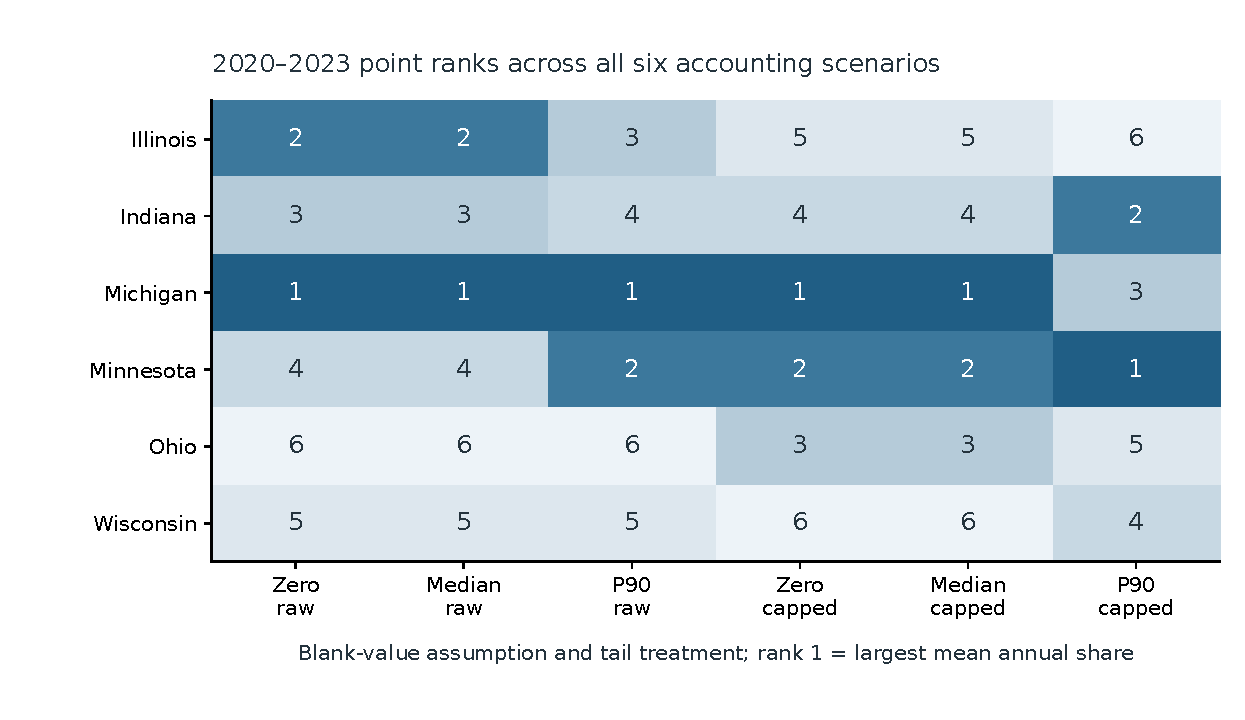
\includegraphics[width=\linewidth]{images/scenario_ranks.pdf}
\captionof{figure}{Every fixed scenario and state, 2020--2023. Numbers are exact point ranks, with darker cells indicating larger reported shares. Median/P90 refer to earlier-period positive values for each event type. The cap applies after blank assignment. These are separate accounting scenarios, not probabilities or estimates of a true-risk interval. Source: minimized NOAA/NWS reports; original calculations.}
\end{center}

The comparator places Michigan first and Illinois second. Assigning the positive median to blanks leaves that ordering unchanged. The uncapped P90 blank scenario moves Minnesota into second place; the capped P90 scenario puts Minnesota first, Indiana second and Michigan third. Thus some point comparisons are stable under modest changes while the declared combined stress can alter even top-two membership.

Across the six scenarios, Illinois ranges from second to sixth, Indiana second to fourth, Michigan first to third, Minnesota first to fourth, Ohio third to sixth and Wisconsin fourth to sixth. No state belongs to the top two in every scenario. Ohio and Wisconsin never enter the top two under these specific conventions; that does not establish low true risk or low unmet need.

Michigan's uncapped blank-as-zero score is 49.1\%, versus 17.5\% in the combined P90/capped case. Illinois changes from 21.4\% to 8.0\%, while Minnesota changes from 7.9\% to 33.1\%. The latter state has 1,126 blank amounts among 3,895 evaluation reports. Assigning a positive value to each blank is consequential and relies on a distributional assumption the records cannot verify.

The score's equal-year weighting is also a deliberate definition. Michigan's uncapped cumulative nominal loss is \$790.7 million, but a cumulative-dollar share and an equal-year share need not agree. The release retains both rather than allowing the label \emph{damage share} to conceal a denominator change.

\newpage
\section*{4. The resampling unit changes apparent precision}
\begin{center}
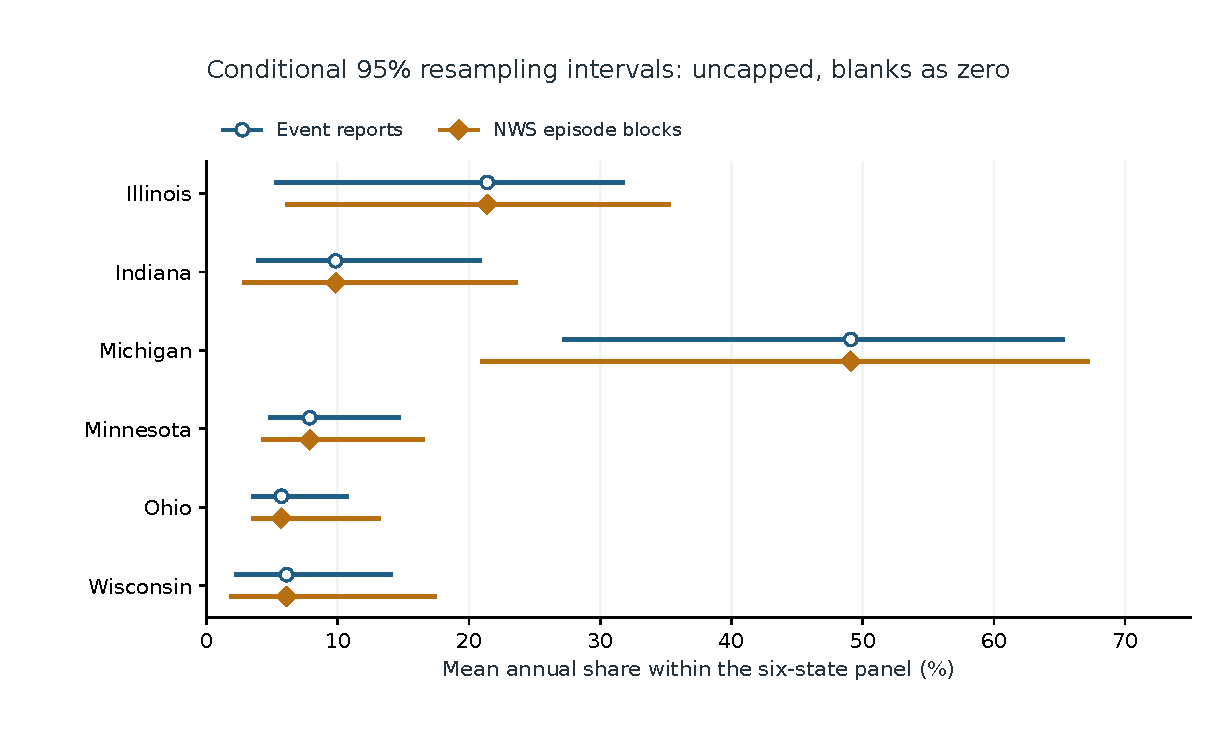
\includegraphics[width=\linewidth]{images/resampling_intervals.pdf}
\captionof{figure}{Conditional central 95\% intervals for the uncapped, blank-as-zero comparator. Points show the original mean annual shares; lines show resampling percentiles. Open circles resample individual reports, diamonds whole NWS episode vectors, within fixed years. Overlap alone is not a test of a state difference; paired contrast outputs are retained. Source: original conditional resampling of the minimized NOAA/NWS panel.}
\end{center}

\begin{center}\small
\begin{tabular}{lrrr}\toprule
State & Event-report width & Episode-block width & Episode top-two frequency\\
 & percentage points & percentage points & \%\\\midrule
Illinois & 26.3 & 29.0 & 75.0\\
Indiana & 16.8 & 20.7 & 17.1\\
Michigan & 37.9 & 46.1 & 98.4\\
Minnesota & 9.7 & 12.1 & 4.8\\
Ohio & 7.1 & 9.5 & 0.8\\
Wisconsin & 11.7 & 15.5 & 3.9\\\bottomrule
\end{tabular}
\captionof{table}{All six intervals widen under episode blocks in this run. Frequencies are conditional on this comparator and the observed reporting process, not probabilities of true-risk rankings. Monte Carlo error and unmodeled reporting selection remain.}
\end{center}

Michigan's event-report interval is [27.3\%, 65.3\%]; its episode-block interval is [21.0\%, 67.1\%]. The evaluation years contain 20,289 report units but only 2,660 episode units. Treating reports within an episode as independent can conceal shared variation. This comparison does not establish that episode blocks remove every dependence source, nor that every interval in every scenario must widen. Complete intervals, ranks and paired comparisons for all six scenarios remain available.

\newpage
\section*{5. Tail treatment reveals year-level influence}
\begin{center}
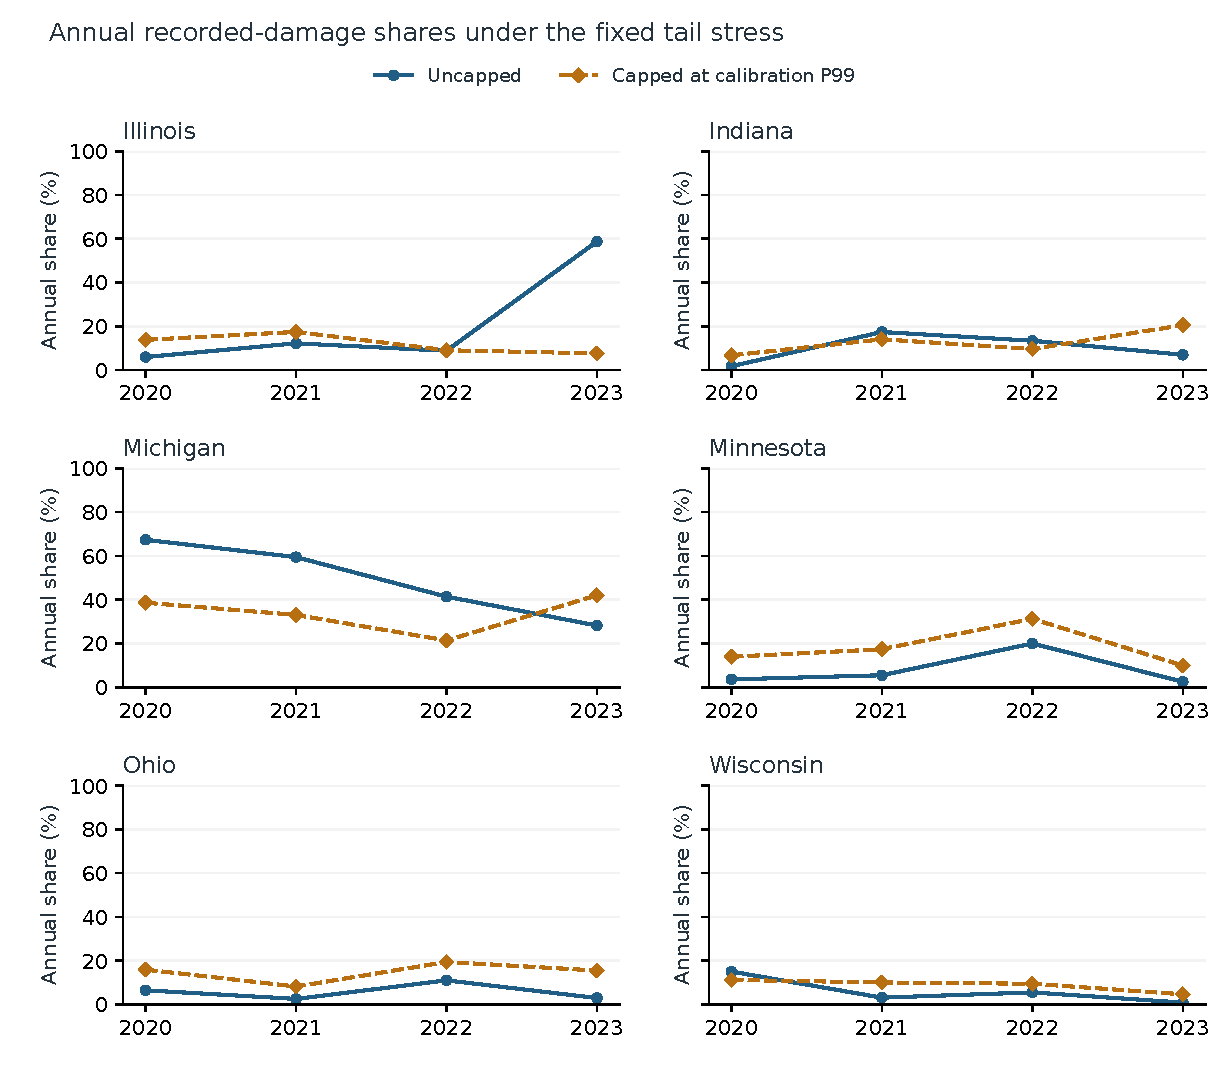
\includegraphics[width=.94\linewidth]{images/annual_tail_sensitivity.pdf}
\captionof{figure}{Every annual share in the uncapped and capped blank-as-zero cases, using a common 0--100\% scale. Each year's denominator includes only the same six states and five event types. The cap is the fixed \$2.791 million calibration threshold, not an inflation adjustment or a correction to official records. Source: minimized NOAA/NWS reports; original calculations.}
\end{center}

Illinois has 58.7\% of the uncapped six-state total in 2023, versus 7.6\% after capping. Omitting 2023 moves its uncapped equal-year rank from second to fourth. Michigan remains first in every uncapped blank-as-zero leave-year-out calculation, even though its point rank changes under the combined reporting/tail stress. These are different robustness questions, and both results are retained.

\newpage
\section*{6. Verification, contribution and remaining uncertainty}
The specific protocol preceded retrieval. Exact minimized source fields were independently compared with all nine private originals; a separate Decimal/parser/SQL path checks every normalized field and all 54 state/year coverage cells. Exact rational order statistics reconstruct all eleven calibrated scenario thresholds. The full calibration-positive export is also checked.

Eight boundary tests cover amount multipliers, missing/zero distinctions, malformed inputs, type-7 interpolation and cent rounding, capping, equal-year weighting, exact ties, undefined denominators and cross-state episode preservation. Scientific code and twelve source/calibration dependencies were committed, hashed and pushed before the first evaluation damage-total, rank or bootstrap command. Only prespecified source coverage/format counts used evaluation rows earlier.

The independent analysis imports no primary helper. SQL constructs annual and unit cent vectors; rational arithmetic reconstructs point and leave-year-out ranks. An indexed-row sum independently checks every primary count-weighted bootstrap annual total. The two implementations share NumPy PCG64; this does not independently certify the RNG library. There are 874,218 independent value checks for development and 738,546 for evaluation, with exact equality for cents and ranks. Floating comparisons retain absolute $10^{-7}$ and relative $10^{-9}$ tolerances. The largest retained floating difference is below $1.7\times10^{-16}$.

A fresh isolated public replay rebuilds 1,855,811 exact cent/discrete fields and 147,422 floating fields from the minimized snapshot. It reruns source, calibration and both analysis paths without fetching a newer vintage. Three original vector figures bind all 120 plotted ranks, endpoints, points and annual values to the checked outputs. The retained manuscript receives separate numerical, hash, active-content and rendered-page checks. Exact-head Linux CI, privacy checks, matching tested/merged trees and an annotated remote tag remain release requirements.

The bounded contribution is a reproducible comparison of reporting assumptions, tail influence and resampling units in this specific panel. Incompleteness in NOAA storm records is already documented; dos Santos examined older data and reported missing amounts and inconsistent labels [5]. Those older missingness rates are not reused as present evidence. No exhaustive literature-gap, new-bootstrap-method, causal or universal scientific-novelty claim is made.

Unreported events, underestimated values and ambiguous zeros remain unidentified. The data lack an exposed-asset denominator and a verified loss-ascertainment model. Four evaluation years are not a stationary future climate sample, and episode grouping is not complete disaster lineage. Conditional intervals and finite scenario ranges cannot replace these missing inputs. No policy or investment should be treated as validated by a single recorded-loss rank.

Full source narratives, precise locations and person-level outcomes are excluded from public history. This manuscript is an independent, AI-assisted research example, not an official NOAA product, journal submission or peer-reviewed result. Separate formal-publication projects, including Azure optimization, remain private.

\newpage
\section*{References and reproducible evidence}
\small
[1] NOAA NCEI. Storm Data bulk CSV format and annual details files. \url{https://www.ncei.noaa.gov/pub/data/swdi/stormevents/csvfiles/Storm-Data-Bulk-csv-Format.pdf}. Index: \url{https://www.ncei.noaa.gov/pub/data/swdi/stormevents/csvfiles/}. Source filenames and hashes are pinned in the retained manifest.

[2] NOAA NCEI. Storm Events Database FAQ. \url{https://www.ncdc.noaa.gov/stormevents/faq.jsp}. Damage estimates, reporting sources, event-year dollars and tornado segmentation; checked 29 October 2026.

[3] National Weather Service. Storm Data Preparation, NWSI 10-1605, damage section. \url{https://www.weather.gov/media/directives/010_pdfs/pd01016005curr.pdf}. Unknown amounts, estimates and the specific flood reporting requirement.

[4] National Weather Service. Data reuse disclaimer. \url{https://www.weather.gov/disclaimer}. See also NCEI Open Data Policy, 14 December 2022, public-domain Federal data and source-specific exceptions: \url{https://www.ncei.noaa.gov/sites/default/files/2023-12/NCEI%20PD-10-2-02%20-%20Open%20Data%20Policy%20Signed.pdf}.

[5] dos Santos, R.P. (2016). \emph{Some comments on the reliability of NOAA's Storm Events Database}. arXiv:1606.06973v2. \url{https://doi.org/10.48550/arXiv.1606.06973}. Exploratory preprint; older database coverage and data-quality findings, not this study's measured rates.

\normalsize
\section*{Files and commands}
Repository: \url{https://github.com/S3R3Bii/storm-damage-ranking}.

\path{data/source/manifest.json} records original and minimized file hashes, extraction rules and timestamps. The public annual subsets retain the exact selected statistical strings and parsed source-row identifiers. \path{results/ORIGINAL_EXTRACTION_CHECK.json} records the private-original comparison without private machine paths or excluded fields.

\path{data/reports.csv} contains the strict cent/blank normalization. \path{results/source_coverage.csv} retains every coverage cell; \path{results/calibration.json} and \path{results/calibration_positives.csv} retain all earlier-period conventions and positive observations. \path{results/CODE_FREEZE.json} binds the protocol, code and input dependencies before evaluation.

\path{results/development/} and \path{results/evaluation/} retain all six scenarios, integer unit vectors, every annual bootstrap total and every replicate/state score and rank, paired comparisons, annual/leave-year-out results, rank frequencies and conditional intervals. Scenario rank envelopes are point-scenario ranges. Original and minimized source validation, numerical reconstruction, figures, manuscript and release checks are separate, scoped evidence gates.

Use Python 3.10 with pinned requirements:
{\small
\begin{verbatim}
python -m unittest discover -s tests -v
python src/check_reproduction.py
python src/verify_figures.py
python src/verify_paper.py
python src/verify_public_package.py
\end{verbatim}
}
The README documents original-source checks and artifact rebuilding.
\end{document}
